\section*{Обработка результатов измерений}

Рассчитаем вектор напряжённости:

$ 
E = \dfrac{d\varphi}{dl} = 
\dfrac{\varDelta \varphi}{\varDelta l}
$\\

$ 
\overline E_x =
\dfrac{\varDelta \varphi}{\varDelta x} =
\dfrac{5.55 - 5.52}{0.005} =
6 \dfrac{B}{m}
$\\

$ 
\overline E_y =
\dfrac{\varDelta \varphi}{\varDelta y} =
\dfrac{5.53 - 5.52}{0.005} =
2 \dfrac{B}{m}
$\\

Рассчитаем погрешность вектора напряжённости:

$ 
\varDelta E = 
\dfrac{\varphi_1 - \varphi_2}{x_1 - x_2}
$\\

$ 
\varDelta E_x = 
\sqrt{
    2(\dfrac{\theta_\varphi}{\varDelta x})^2 + 
    2(\dfrac{\varDelta \varphi \theta_l}{\varDelta x ^2})^2
} = 
\sqrt{
    2(\dfrac{0.01}{0.005})^2 + 
    2(\dfrac{0.03 * 0.001}{0.000025})^2
} = 
3,3
$\\

$ 
\varDelta E_y = 
\sqrt{
    2(\dfrac{\theta_\varphi}{\varDelta y})^2 + 
    2(\dfrac{\varDelta \varphi \theta_l}{\varDelta y ^2})^2
} = 
\sqrt{
    2(\dfrac{0.01}{0.005})^2 + 
    2(\dfrac{0.03 * 0.001}{0.000025})^2
} = 
2,9
$\\

$ 
E = 
\sqrt{
    E_x^2 + E_y^2 
} = 6.3 \pm 4.3
$\\

Рассчитаем касательные составляющие для отрезков выбранного контура:\\ 

% E 1 #########################
$
E_{1} = 
\dfrac{\varDelta \varphi}{\varDelta l} =
\dfrac{7.31 - 7.01}{0.004} = 
75.0
$\\


% E 2 #########################
$
E_{2} = 
\dfrac{\varDelta \varphi}{\varDelta l} =
\dfrac{7.73 - 7.5}{0.004} = 
57.5
$\\


% E 3 #########################
$
E_{3} = 
\dfrac{\varDelta \varphi}{\varDelta l} =
\dfrac{8.02 - 7.98}{0.004} = 
10.0
$\\


% E 4 #########################
$
E_{4} = 
\dfrac{\varDelta \varphi}{\varDelta l} =
\dfrac{8.16 - 8.18}{0.004} = 
-5.0
$\\


% E 5 #########################
$
E_{5} = 
\dfrac{\varDelta \varphi}{\varDelta l} =
\dfrac{8.06 - 8.25}{0.004} = 
-47.5
$\\


% E 6 #########################
$
E_{6} = 
\dfrac{\varDelta \varphi}{\varDelta l} =
\dfrac{8.0 - 8.12}{0.004} = 
-30.0
$\\


% E 7 #########################
$
E_{7} = 
\dfrac{\varDelta \varphi}{\varDelta l} =
\dfrac{7.77 - 7.94}{0.004} = 
-42.5
$\\


% E 8 #########################
$
E_{8} = 
\dfrac{\varDelta \varphi}{\varDelta l} =
\dfrac{7.44 - 7.69}{0.004} = 
-62.5
$\\


% E 9 #########################
$
E_{9} = 
\dfrac{\varDelta \varphi}{\varDelta l} =
\dfrac{7.04 - 7.25}{0.004} = 
-52.5
$\\


% E 10 #########################
$
E_{10} = 
\dfrac{\varDelta \varphi}{\varDelta l} =
\dfrac{6.65 - 6.95}{0.004} = 
-75.0
$\\


% E 11 #########################
$
E_{11} = 
\dfrac{\varDelta \varphi}{\varDelta l} =
\dfrac{6.53 - 6.55}{0.004} = 
-5.0
$\\


% E 12 #########################
$
E_{12} = 
\dfrac{\varDelta \varphi}{\varDelta l} =
\dfrac{6.2 - 6.44}{0.004} = 
-60.0
$\\


% E 13 #########################
$
E_{13} = 
\dfrac{\varDelta \varphi}{\varDelta l} =
\dfrac{6.14 - 6.17}{0.004} = 
-7.5
$\\


% E 14 #########################
$
E_{14} = 
\dfrac{\varDelta \varphi}{\varDelta l} =
\dfrac{6.04 - 6.1}{0.004} = 
-15.0
$\\


% E 15 #########################
$
E_{15} = 
\dfrac{\varDelta \varphi}{\varDelta l} =
\dfrac{6.04 - 6.17}{0.004} = 
-32.5
$\\


% E 16 #########################
$
E_{16} = 
\dfrac{\varDelta \varphi}{\varDelta l} =
\dfrac{6.13 - 6.08}{0.004} = 
12.5
$\\


% E 17 #########################
$
E_{17} = 
\dfrac{\varDelta \varphi}{\varDelta l} =
\dfrac{6.63 - 6.47}{0.004} = 
40.0
$\\


% E 18 #########################
$
E_{18} = 
\dfrac{\varDelta \varphi}{\varDelta l} =
\dfrac{6.91 - 6.81}{0.004} = 
25.0
$\\

\begin{figure}
    \centering
    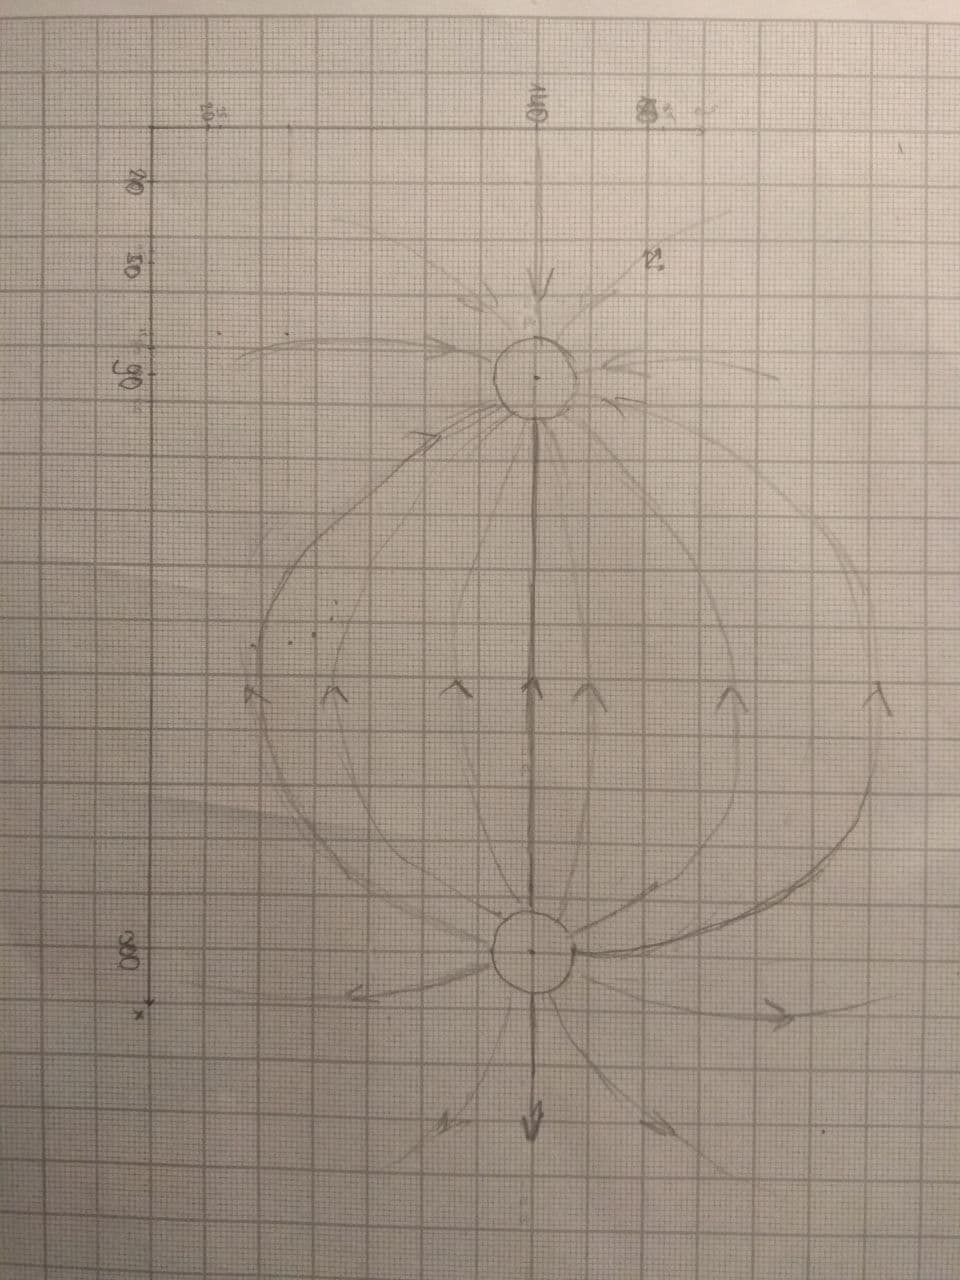
\includegraphics[width=\linewidth,angle=180]{photo/s}
\end{figure}



